\section{State Observer Based on Particle Filter}

\subsection{Particle filter algorithm}

The specific steps of the particle filter algorithm are as Figure 2. Steps three, four, and five are repeated to achieve recursion.

\begin{figure}
    \centering
    
    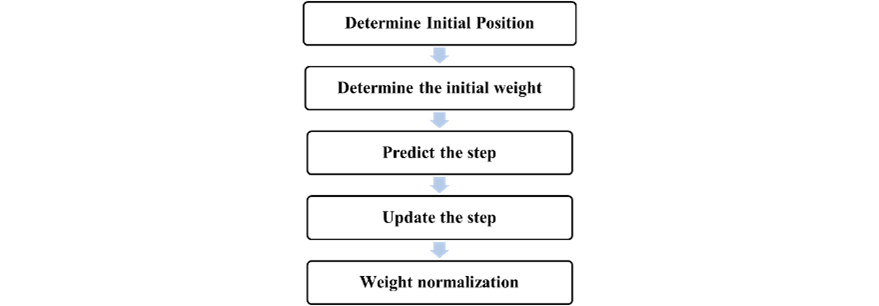
\includegraphics{Sensor_Fusion_pictures/figure2.png}
    \caption{Steps of particle filter algorithm.}
    \label{stepsOfAlgorithm}
\end{figure}

The triggering methods of resampling are divided into periodic triggering and threshold triggering. Threshold triggering refers to triggering resampling when the ratio of the effective particle number to the total particle number is lower than the set threshold. The number of effective particles can be approximated as:

\begin{equation}
    
\end{equation}